% 贡献者：汤立祥
\heading{数学物理方法（上）-第1次作业}


\begin{question}
由 \(2\times 2\) 实矩阵组成的集合
\[
\left\{\begin{pmatrix} x & y \\ -y & x \end{pmatrix}:\; x\in\mathbb{R},\; y\in\mathbb{R}\right\}
\]
其中矩阵之间的加法和乘法满足线性代数中介绍的通常的矩阵运算规则。
证明这个集合构成一个域，且与复数域同构。
\begin{solution}
记上述集合为 \(S\)，我们首先证明上述集合构成域。

加、乘\textbf{封闭性}是容易证明的。任取
\[
A_j=\begin{pmatrix}x_j&y_j\\-y_j&x_j\end{pmatrix}\in S,
\qquad j=1,2.
\]
\[
\begin{pmatrix} x_1 & y_1 \\ -y_1 & x_1 \end{pmatrix}
+\begin{pmatrix} x_2 & y_2 \\ -y_2 & x_2 \end{pmatrix}
=\begin{pmatrix} x_1+x_2 & y_1+y_2 \\ -y_1-y_2 & x_1+x_2 \end{pmatrix}\in S,
\]
\[
\begin{pmatrix} x_1 & y_1 \\ -y_1 & x_1 \end{pmatrix}
\begin{pmatrix} x_2 & y_2 \\ -y_2 & x_2 \end{pmatrix}
=\begin{pmatrix} x_1x_2-y_1y_2 & x_2y_1+x_1y_2 \\ -x_2y_1-x_1y_2 & x_1x_2-y_1y_2 \end{pmatrix}\in S.
\]

对于\textbf{加法}而言：
\begin{enumerate}
  \item 有加法单位元 \(\mathbf{0}:=\begin{pmatrix}0&0\\0&0\end{pmatrix}\in S\)，
  对任意 \(A=\begin{pmatrix}x&y\\-y&x\end{pmatrix}\in S\)，有
  \[
  A+\mathbf0=\mathbf0+A=A.
  \]
  \item 对于任意 \(\begin{pmatrix}x&y\\-y&x\end{pmatrix}\in S\)，
  都有逆元 \(\begin{pmatrix}-x&-y\\y&-x\end{pmatrix}\in S\)，此时
  \[
  \begin{pmatrix}x&y\\-y&x\end{pmatrix}+\begin{pmatrix}-x&-y\\y&-x\end{pmatrix}
  =\begin{pmatrix}-x&-y\\y&-x\end{pmatrix}+\begin{pmatrix}x&y\\-y&x\end{pmatrix}
  =\mathbf{0};
  \]
  \item 显然具有结合律和交换律。
\end{enumerate}

对于\textbf{乘法}而言：
\begin{enumerate}
  \item 有乘法单位元 \(\mathbf{1}:=\begin{pmatrix}1&0\\0&1\end{pmatrix}\in S\)，
  注意到
  \[
  \begin{pmatrix}1&0\\0&1\end{pmatrix}\begin{pmatrix}x&y\\-y&x\end{pmatrix}
  =\begin{pmatrix}x&y\\-y&x\end{pmatrix}\begin{pmatrix}1&0\\0&1\end{pmatrix}
  =\begin{pmatrix}x&y\\-y&x\end{pmatrix}
  \]
  不变；
  \item 对于任意 \(\begin{pmatrix}x&y\\-y&x\end{pmatrix}\in S\setminus\{\mathbf{0}\}\)，
  都有逆元
  \[
  \frac{1}{x^2+y^2}\begin{pmatrix}x&-y\\y&x\end{pmatrix}\in S\setminus\{\mathbf{0}\},
  \]
  此时
  \[
  \frac{1}{x^2+y^2}\begin{pmatrix}x&-y\\y&x\end{pmatrix}
  \begin{pmatrix}x&y\\-y&x\end{pmatrix}
  =\begin{pmatrix}x&y\\-y&x\end{pmatrix}
  \frac{1}{x^2+y^2}\begin{pmatrix}x&-y\\y&x\end{pmatrix}
  =\mathbf{1};
  \]
  \item 对于交换律，\(\forall\begin{pmatrix}a&b\\-b&a\end{pmatrix},
  \begin{pmatrix}c&d\\-d&c\end{pmatrix}\in S\)：
  \[
  \begin{pmatrix}a&b\\-b&a\end{pmatrix}
  \begin{pmatrix}c&d\\-d&c\end{pmatrix}
  =\begin{pmatrix}ac-bd&bc+ad\\-bc-ad&ac-bd\end{pmatrix},
  \]
  \[
  \begin{pmatrix}c&d\\-d&c\end{pmatrix}
  \begin{pmatrix}a&b\\-b&a\end{pmatrix}
  =\begin{pmatrix}ac-bd&bc+ad\\-bc-ad&ac-bd\end{pmatrix};
  \]
  \item 显然具有结合律。
\end{enumerate}

由矩阵的性质，其自身显然满足分配律。由此我们证明了 \(S\) 在矩阵加法与矩阵乘法下构成域。

我们再来证明其与复数域 \(\mathbb{C}\) 同构。

定义从 \(S\) 到复数域 \(\mathbb{C}\) 的映射
\[
f\!\left(\begin{pmatrix}x&y\\-y&x\end{pmatrix}\right)=x+\ii y,
\]
对任意
\[
A_j=\begin{pmatrix}x_j&y_j\\-y_j&x_j\end{pmatrix}\in S,
\qquad j=1,2,
\]
\[
\begin{aligned}
f\!\left(\begin{pmatrix}x_1&y_1\\-y_1&x_1\end{pmatrix}
+\begin{pmatrix}x_2&y_2\\-y_2&x_2\end{pmatrix}\right)
&=(x_1+x_2)+\ii(y_1+y_2)\\
&=f\!\left(\begin{pmatrix}x_1&y_1\\-y_1&x_1\end{pmatrix}\right)
+f\!\left(\begin{pmatrix}x_2&y_2\\-y_2&x_2\end{pmatrix}\right),\\[4pt]
f\!\left(\begin{pmatrix}x_1&y_1\\-y_1&x_1\end{pmatrix}
\begin{pmatrix}x_2&y_2\\-y_2&x_2\end{pmatrix}\right)
&=(x_1x_2-y_1y_2)+\ii(x_1y_2+x_2y_1)\\
&=f\!\left(\begin{pmatrix}x_1&y_1\\-y_1&x_1\end{pmatrix}\right)
\cdot f\!\left(\begin{pmatrix}x_2&y_2\\-y_2&x_2\end{pmatrix}\right).
\end{aligned}
\]

由此我们证明了 \(S\) 与复数域 \(\mathbb{C}\) 同构。
\end{solution}
\end{question}


\begin{question}
计算下列表达式的值：\((1+\ii)^{-n}+(1-\ii)^{n}\)，其中 \(n\) 为整数。
\begin{solution}
\[
(1+\ii)^{-n}+(1-\ii)^{n}
= \sqrt{2}^{\,-n}\ee^{-\ii n\pi/4} + \sqrt{2}^{\,n}\ee^{-\ii n\pi/4}
= \bigl(2^{n/2}+2^{-n/2}\bigr)\ee^{-\ii n\pi/4}.
\]
\end{solution}
\end{question}


\begin{question}
写出复数 \(\ee^{-z}\) 的实部、虚部、模和辐角。
\begin{solution}
设 \(z=x+\ii y,\;x,y\in\mathbb{R}\)，则有
\[
\ee^{-z}=\ee^{-x}(\cos y+\ii\sin y).
\]
所以有
\[
\operatorname{Re}\ee^{-z}=\ee^{-x}\cos y,\qquad
\operatorname{Im}\ee^{-z}=\ee^{-x}\sin y,
\]
\[
|\ee^{-z}|=\ee^{-x},\qquad
\arg\ee^{-z}=y.
\]
\end{solution}
\end{question}


\begin{question}
把下列关系用几何图形表示出来：

\begin{enumerate}
  \item \(\displaystyle\operatorname{Re}\frac{z-z_1}{z-z_2}=0\)；
  \item \(|1-z^2|<|2z|\)；
  \item \(\displaystyle 0<\arg\frac{z+\ii}{z-\ii}<\frac{\pi}{4}\)。
\end{enumerate}
\begin{solution}
\begin{enumerate}
  \item 取 \(\lambda\in\mathbb{R}\)，有 \(z-z_1=\lambda\ii(z-z_2)\)，
  即意味着 \(\arg(z-z_1)=\arg(z-z_2)+\pi/2\)，
  所以有线段 \(\overline{zz_1}\perp\overline{zz_2}\)，
  \(z\) 位于以 \(z_1,z_2\) 为直径的圆上。

  \begin{center}
  \begin{tikzpicture}[scale=0.8]
    \draw[->] (-1,0) -- (3,0) node[right] {\(x\)};
    \draw[->] (0,-1) -- (0,2.5) node[above] {\(y\)};
    \draw (1,0.5) circle ({sqrt(5/4)});
    \filldraw (0,0) circle (2pt) node[below right] {\(z_1\)};
    \filldraw[fill=white] (2,1) circle (2pt) node[below right] {\(z_2\)};
  \end{tikzpicture}
  \end{center}

  \item 设 \(z=r\ee^{\ii\theta},\;r,\theta\in\mathbb{R}\)，
  有 \(|1-z^2|=\sqrt{1+r^4-2r^2\cos2\theta}\)，\(|2z|=2r\)。
  即需要解不等式
  \[
  \sqrt{1+r^4-2r^2\cos2\theta}<2r,
  \]
  即
  \[
  r^4-2r^2(\cos2\theta+2)+1<0.
  \]
  解得
  \[
  \sqrt{2+\cos2\theta-\sqrt{3+4\cos2\theta+\cos^2\!2\theta}}
  <r<
  \sqrt{2+\cos2\theta+\sqrt{3+4\cos2\theta+\cos^2\!2\theta}}.
  \]
  可以看到是一个条带。为了更好看清边界的方程，考察 \(|1-z^2|=|2z|\) 的区域，
  设 \(z=x+\ii y,\;x,y\in\mathbb{R}\)，则
  \[
  4(x^2+y^2)=(1-x^2+y^2)^2+4x^2y^2,
  \]
  即
  \[
  1-6x^2+x^4+(-2+2x^2)y^2+y^4=0.
  \]
  因式分解可以得到
  \[
  \bigl((x-1)^2+y^2-2\bigr)\bigl((x+1)^2+y^2-2\bigr)=0.
  \]
  可以看到是两个圆。

  \begin{center}
    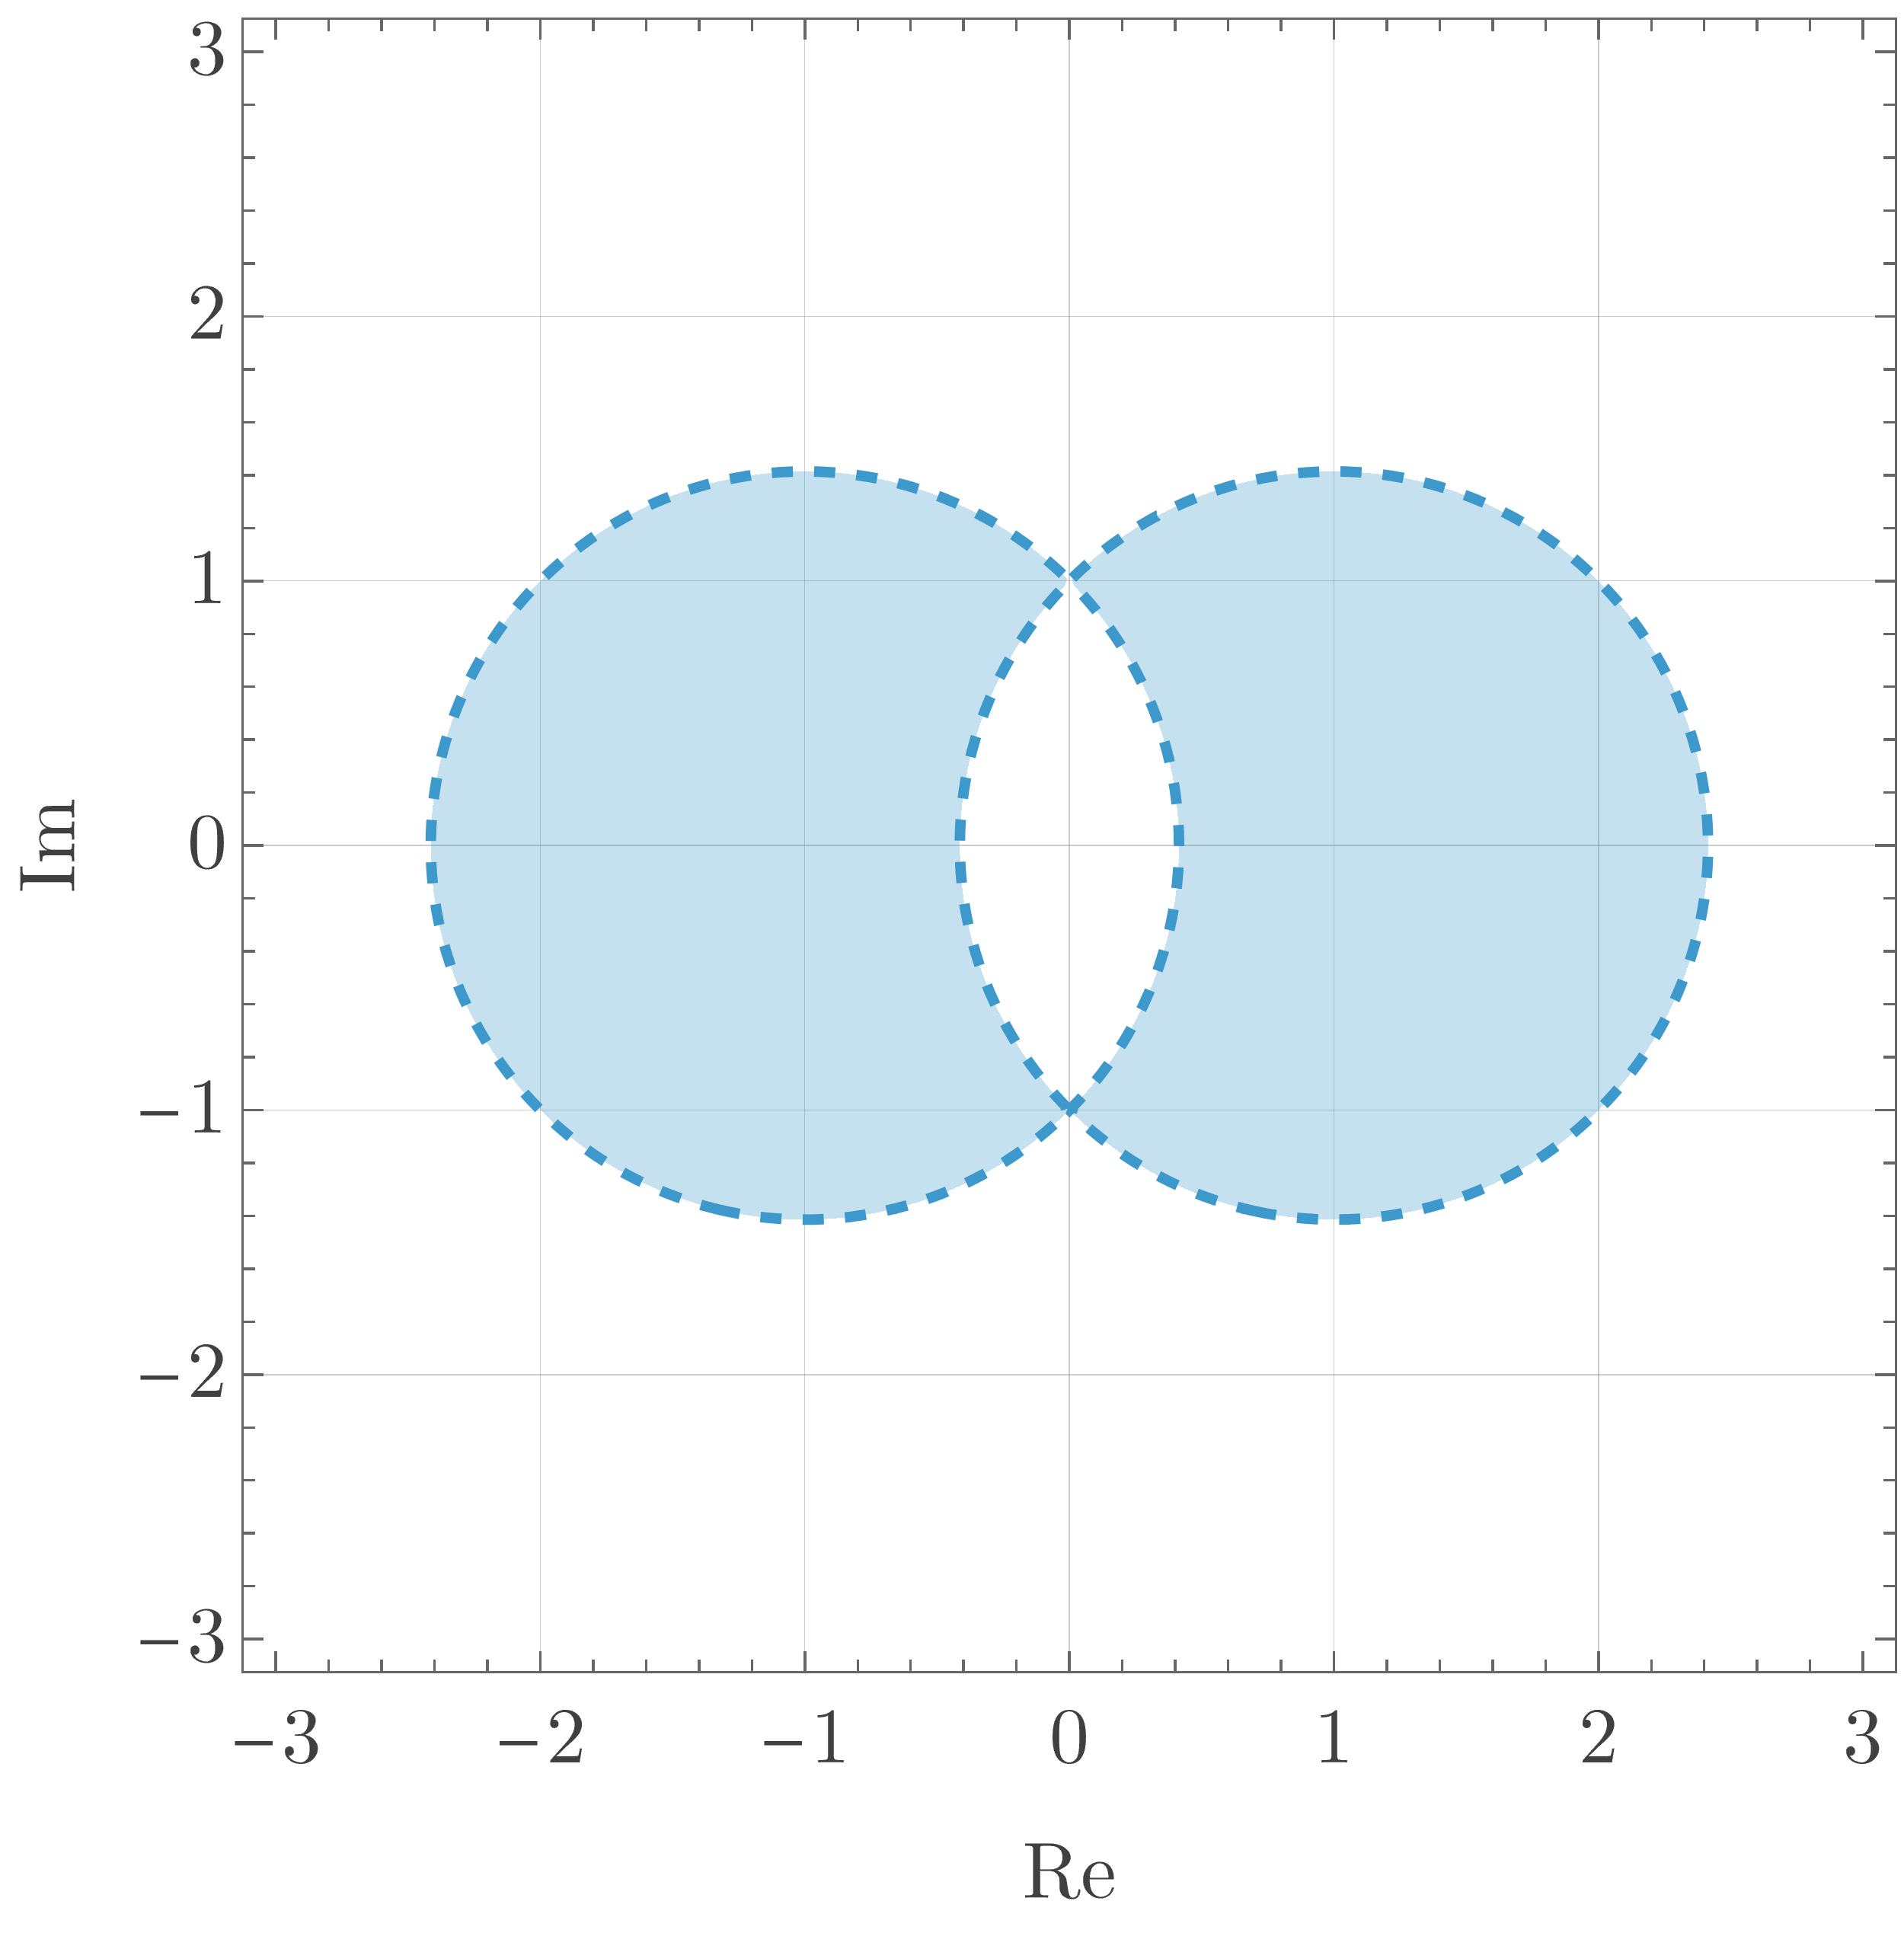
\includegraphics[width=0.35\linewidth]{figures/第1次作业-fig01.png}
  \end{center}

  \item 有 \(\displaystyle\arg\frac{z+\ii}{z-\ii}=\arg(z+\ii)-\arg(z-\ii)\)，
  即 \(\overline{z\ii},\;\overline{z(-\ii)}\) 之间的夹角小于 \(\pi/4\)。
  当 \(\overline{z\ii},\;\overline{z(-\ii)}\) 夹角恒定时，划过的曲线为一圆弧，
  若夹角为 \(\alpha\)，则 \(\overline{\ii(-\ii)}\) 段对应的圆心角为 \(2\alpha\)。
  通过符号判断可知实际的边界为另一边圆心角为 \(2\pi-2\alpha\)，
  因此最后结果是虚轴的一部分与一圆心角为 \(3\pi/2\) 圆弧围成的区域。

  \begin{center}
    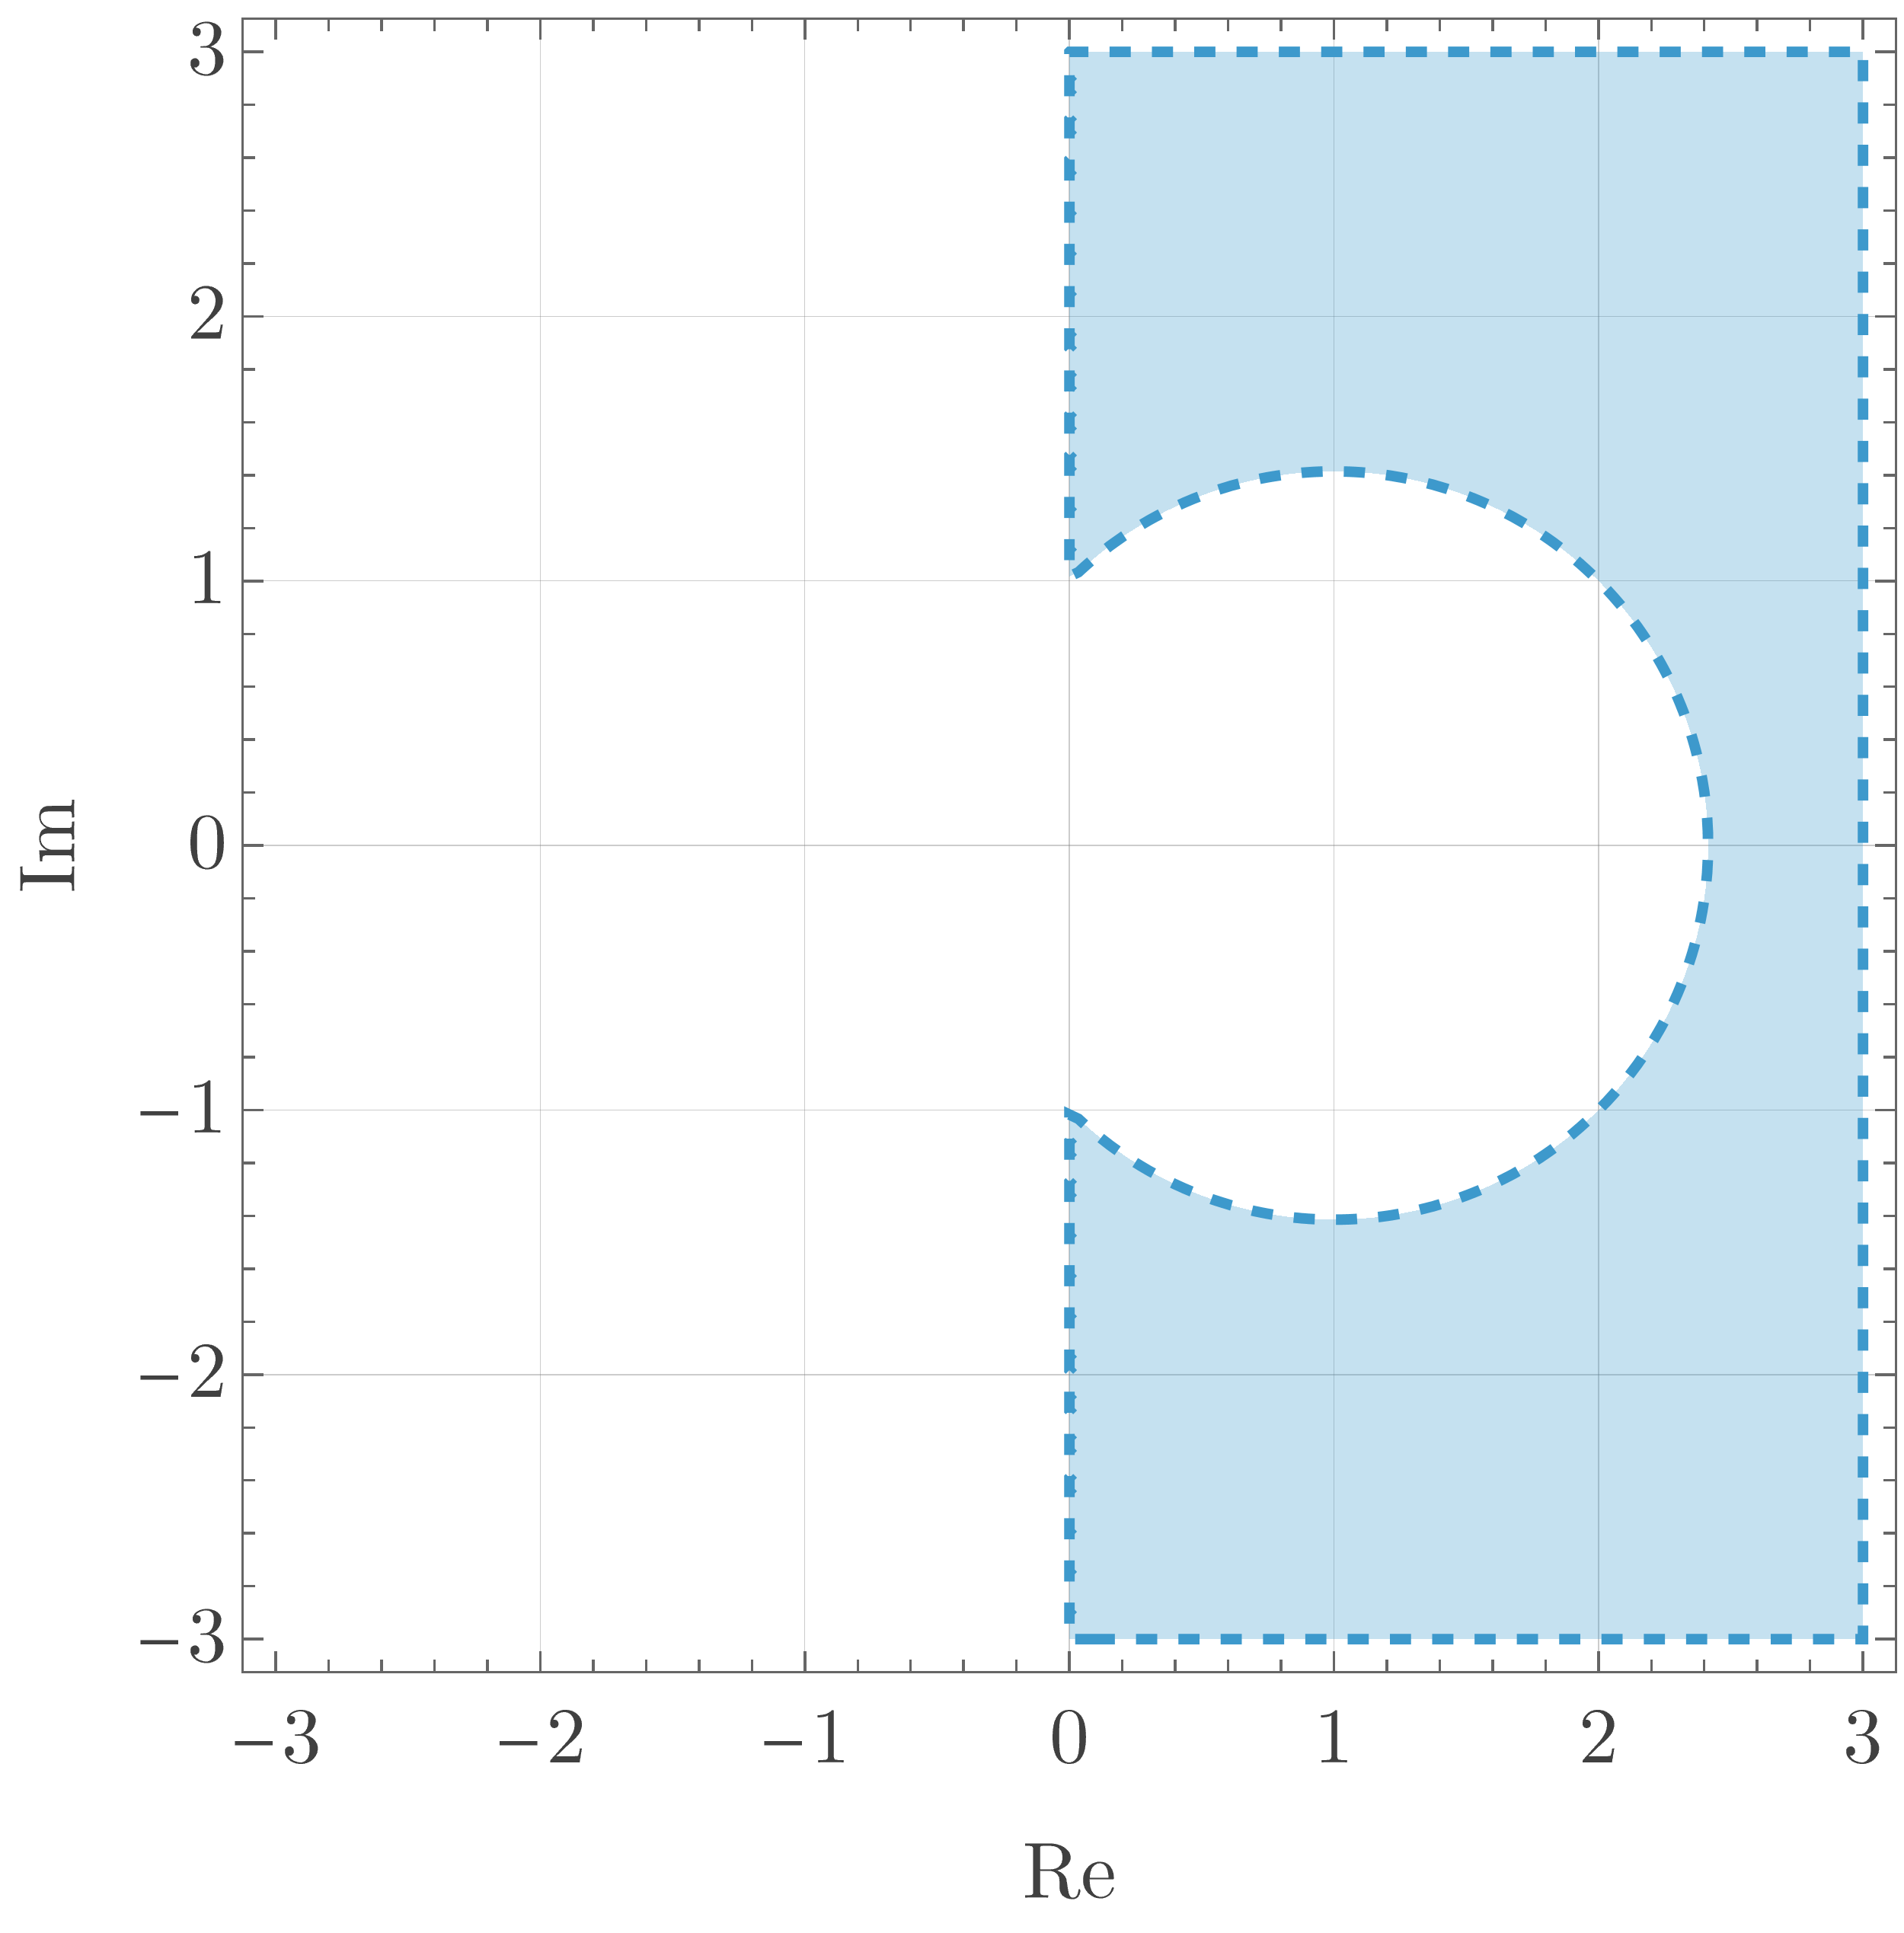
\includegraphics[width=0.35\linewidth]{figures/第1次作业-fig02.png}
  \end{center}
\end{enumerate}
\end{solution}
\end{question}


\begin{question}
已知一复数 \(z\)，请画出 \(\ii z\)、\(-z\)、\(z^*\)、\(1/z\) 和 \(1/z^*\)，
并指出它们之间的几何关系。
\begin{solution}
设 \(z=r\ee^{\ii\theta}\)，则：
\begin{enumerate}
  \item \(\ii z=\ee^{\ii\pi/2}z\)，即将 \(z\) 绕原点逆时针旋转 \(\pi/2\)；
  \item \(-z=\ee^{\ii\pi}z\)，即将 \(z\) 绕原点旋转 \(\pi\)；
  \item \(z^*=r\ee^{-\ii\theta}\)，即 \(z\) 关于实轴的对称点；
  \item \(\displaystyle\frac{1}{z}=\frac{1}{r}\ee^{-\ii\theta}\)，即 \(z\) 关于实轴对称后关于原点缩放 \(1/r^2\)；
  \item \(\displaystyle\frac{1}{z^*}=\frac{1}{r}\ee^{\ii\theta}\)，即 \(z\) 关于原点缩放 \(1/r^2\)。
\end{enumerate}

各点的位置关系如图所示：

\begin{center}
\begin{tikzpicture}[scale=1.5]
  \draw[->] (-2,0) -- (2.5,0) node[right] {\(\operatorname{Re}\)};
  \draw[->] (0,-2) -- (0,2.5) node[above] {\(\operatorname{Im}\)};
  \draw[dashed] (0,0) circle (1);
  \filldraw (1.5,1) circle (1.5pt) node[below right] {\(z\)};
  \draw[thin] (0,0) -- (1.5,1);
  \filldraw (-1,1.5) circle (1.5pt) node[below right] {\(\ii z\)};
  \draw[thin] (0,0) -- (-1,1.5);
  \filldraw (-1.5,-1) circle (1.5pt) node[below left] {\(-z\)};
  \draw[thin] (0,0) -- (-1.5,-1);
  \filldraw (1.5,-1) circle (1.5pt) node[above right] {\(z^*\)};
  \draw[thin] (0,0) -- (1.5,-1);
  \filldraw (0.4615,-0.3077) circle (1.5pt)
    node[below right=3pt] {\(1/z\)};
  \draw[thin] (0,0) -- (0.4615,-0.3077);
  \filldraw (0.4615,0.3077) circle (1.5pt)
    node[above right=3pt] {\(1/z^*\)};
  \draw[thin] (0,0) -- (0.4615,0.3077);
  \node at (1,0) [below right] {\(1\)};
  \node at (0,1) [below right] {\(i\)};
\end{tikzpicture}
\end{center}
\end{solution}
\end{question}


\begin{question}
求下列序列 \(z_n\) 的聚点和极限，如果是实数序列，则同时求出上极限和下极限：
\begin{enumerate}
  \item \(\displaystyle z_n=\Bigl(1+\frac{\ii}{n}\Bigr)\sin\frac{n\pi}{6}\)；
  \item \(\displaystyle z_n=\Bigl(1+\frac{1}{2n}\Bigr)\cos\frac{n\pi}{3}\)。
\end{enumerate}
\begin{solution}
\begin{enumerate}
  \item 容易看出，当 \(n\to\infty\) 时，\(\dfrac{\ii}{n}\to0\)，
  因此聚点为 \(0,\pm\dfrac12,\pm\dfrac{\sqrt3}{2},\pm1\)，不存在极限。
  \item 容易看出，当 \(n\to\infty\) 时，\(\dfrac{1}{2n}\to0\)，
  因此聚点为 \(\pm\dfrac12,\pm1\)，上极限为 \(1\)，下极限为 \(-1\)。
\end{enumerate}
\end{solution}
\end{question}


\begin{question}
试求从坐标原点到曲线 \(|z+1/z|=a\) 上各点的最大与最小距离。
\begin{solution}
设 \(z=r\ee^{\ii\theta},\;r,\theta\in\mathbb{R}\)，则有
\[
\bigl|z+1/z\bigr|
=\bigl|r\ee^{\ii\theta}+r^{-1}\ee^{-\ii\theta}\bigr|
=\sqrt{r^2+r^{-2}+2\cos2\theta}.
\]
因此可以得到
\[
r^2+r^{-2}=a^2-2\cos2\theta.
\]
根据 \(r^2+r^{-2}\) 的图像，可以知道当 \(\theta=\pm\pi/2\) 时，
上式的解 \(r_1,r_2\) 分别为最大值与最小值，有
\[
r_{\max}=\frac12\bigl(a+\sqrt{4+a^2}\bigr),\qquad
r_{\min}=\frac12\bigl(-a+\sqrt{4+a^2}\bigr).
\]
\end{solution}
\end{question}


\begin{question}
可否适当选取常数 \(A\)，使得函数
\[
f(z)=\begin{cases}
\dfrac{[\operatorname{Re}(z^2)]^2}{z^2}, & z\neq0,\\[6pt]
A, & z=0
\end{cases}
\]
在 \(z=0\) 点连续。
\begin{solution}
设 \(z=r\ee^{\ii\theta},\;r,\theta\in\mathbb{R}\)，有当 \(r\neq0\) 时，
\[
f(z)=\frac{(r^2\cos2\theta)^2}{r^2\ee^{2\ii\theta}}
=r^2\frac{\cos^2\!2\theta}{\ee^{2\ii\theta}}.
\]

我们可以取 \(A=0\)，此时在 \(z=0\) 处，
\(\forall\varepsilon>0\)，取 \(\delta<\varepsilon^{1/2}\)，
此时 \(\forall|z-0|=r<\delta\)，都有
\[
|f(z)-f(0)|
=\Bigl|r^2\frac{\cos^2\!2\theta}{\ee^{2\ii\theta}}\Bigr|
\le r^2<\delta^2<\varepsilon.
\]
由此可知，\(f(z)\) 在 \(z=0\) 处连续，\(A\) 应取 \(0\)。
\end{solution}
\end{question}


\begin{question}
判断下列函数在何处可导（并求出其导数），在何处解析：
\begin{enumerate}
  \item \(|z|,\)
  \item \(z^*,\)
  \item \(z\cdot\operatorname{Re}z,\)
  \item \((x^2+2y)+\ii(x^2+y^2),\)
  \item \(3x^2+2\ii y^3,\)
  \item \((x-y)^2+2\ii(x+y).\)
\end{enumerate}
\begin{solution}
\begin{enumerate}
  \item 由题，\(u(x,y)=\sqrt{x^2+y^2},\;v(x,y)=0\)。
  当 \(x=y=0\) 时，\(u(x,y)\) 导数不存在。
  在其余区域，
  \[
  \frac{\partial u}{\partial x}=\frac{x}{\sqrt{x^2+y^2}},\quad
  \frac{\partial v}{\partial y}=0\quad\Longrightarrow\quad
  \frac{\partial u}{\partial x}\neq\frac{\partial v}{\partial y},
  \]
  \[
  \frac{\partial u}{\partial y}=\frac{y}{\sqrt{x^2+y^2}},\quad
  \frac{\partial v}{\partial x}=0\quad\Longrightarrow\quad
  \frac{\partial u}{\partial y}\neq-\frac{\partial v}{\partial x}.
  \]
  显然不满足柯西—黎曼条件，故处处不可导，处处不解析。

  \item 由题，\(u(x,y)=x,\;v(x,y)=-y\)。
  在全空间上 \(u,v\) 关于 \(x,y\) 的偏导数都存在，但
  \[
  \frac{\partial u}{\partial x}=1,\quad
  \frac{\partial v}{\partial y}=-1\quad\Longrightarrow\quad
  \frac{\partial u}{\partial x}\neq\frac{\partial v}{\partial y},
  \]
  \[
  \frac{\partial u}{\partial y}=0,\quad
  \frac{\partial v}{\partial x}=0\quad\Longrightarrow\quad
  \frac{\partial u}{\partial y}=-\frac{\partial v}{\partial x}.
  \]
  显然不满足柯西—黎曼条件，故处处不可导，处处不解析。

  \item 由题，\(u(x,y)=x^2,\;v(x,y)=xy\)。
  在全空间上 \(u,v\) 关于 \(x,y\) 的偏导数都存在，但
  \[
  \frac{\partial u}{\partial x}=2x,\quad
  \frac{\partial v}{\partial y}=x\quad\Longrightarrow\quad
  \frac{\partial u}{\partial x}=\frac{\partial v}{\partial y}\ \text{只在}\ x=0\ \text{成立},
  \]
  \[
  \frac{\partial u}{\partial y}=0,\quad
  \frac{\partial v}{\partial x}=y\quad\Longrightarrow\quad
  \frac{\partial u}{\partial y}=-\frac{\partial v}{\partial x}\ \text{只在}\ y=0\ \text{成立}.
  \]
  \(f(z)\) 只在 \(z=0\) 处满足柯西—黎曼条件，
  容易验证其在 \(z=0\) 可导，此点处导数为 \(0\)，处处不解析。

  \item 由题，\(u(x,y)=x^2+2y,\;v(x,y)=x^2+y^2\)。
  在全空间上 \(u,v\) 关于 \(x,y\) 的偏导数都存在，但
  \[
  \frac{\partial u}{\partial x}=2x,\quad
  \frac{\partial v}{\partial y}=2y\quad\Longrightarrow\quad
  \frac{\partial u}{\partial x}=\frac{\partial v}{\partial y}\ \text{只在}\ x=y\ \text{成立},
  \]
  \[
  \frac{\partial u}{\partial y}=2,\quad
  \frac{\partial v}{\partial x}=2y\quad\Longrightarrow\quad
  \frac{\partial u}{\partial y}=-\frac{\partial v}{\partial x}\ \text{只在}\ y=-1\ \text{成立}.
  \]
  因此 \(f(z)\) 只在 \(z=-1-\ii\) 处满足柯西—黎曼条件，
  容易验证其在 \(z=-1-\ii\) 处可导，此点处导数为 \(-2-2\ii\)，处处不解析。

  \item 由题，\(u(x,y)=3x^2,\;v(x,y)=2y^3\)。
  在全空间上 \(u,v\) 关于 \(x,y\) 的偏导数都存在，但
  \[
  \frac{\partial u}{\partial x}=6x,\quad
  \frac{\partial v}{\partial y}=6y^2\quad\Longrightarrow\quad
  \frac{\partial u}{\partial x}=\frac{\partial v}{\partial y}\ \text{只在}\ x=y^2\ \text{成立},
  \]
  \[
  \frac{\partial u}{\partial y}=0,\quad
  \frac{\partial v}{\partial x}=0\quad\Longrightarrow\quad
  \frac{\partial u}{\partial y}=-\frac{\partial v}{\partial x}.
  \]
  因此 \(f(z)\) 只在 \(x=y^2\) 上满足柯西—黎曼条件，
  容易验证其在 \(x=y^2\) 处可导。由
  \(f'(z)=u_x+\ii v_x\)，导数为 \(6x=6y^2\)，处处不解析。

  \item 由题，\(u(x,y)=(x-y)^2,\;v(x,y)=2(x+y)\)。
  在全空间上 \(u,v\) 关于 \(x,y\) 的偏导数都存在，但
  \[
  \frac{\partial u}{\partial x}=2(x-y),\quad
  \frac{\partial v}{\partial y}=2\quad\Longrightarrow\quad
  \frac{\partial u}{\partial x}=\frac{\partial v}{\partial y}\ \text{只在}\ x-y=1\ \text{成立},
  \]
  \[
  \frac{\partial u}{\partial y}=-2(x-y),\quad
  \frac{\partial v}{\partial x}=2\quad\Longrightarrow\quad
  \frac{\partial u}{\partial y}=-\frac{\partial v}{\partial x}\ \text{只在}\ x-y=1\ \text{成立}.
  \]
  因此 \(f(z)\) 只在 \(x-y=1\) 上满足柯西—黎曼条件，
  容易验证其在 \(x-y=1\) 处可导，导数为 \(2(x-y)+2\ii\)，处处不解析。
\end{enumerate}
\end{solution}
\end{question}


\begin{question}
证明平面极坐标系 \((\rho,\phi)\) 下的 Cauchy—Riemann 方程：
\[
\frac{\partial u}{\partial\rho}=\frac{1}{\rho}\frac{\partial v}{\partial\phi},\qquad
\frac{\partial v}{\partial\rho}=-\frac{1}{\rho}\frac{\partial u}{\partial\phi},
\]
其中 \(u(\rho,\phi)\) 和 \(v(\rho,\phi)\) 分别是一个复变函数 \(f\) 的实部和虚部。
\begin{solution}
由题，有 \(f(\rho,\phi)=u(\rho,\phi)+\ii v(\rho,\phi)\)，
因此有 \(\Delta z=\Delta\rho\,\ee^{\ii\phi}+\ii\rho\Delta\phi\,\ee^{\ii\phi}\)。
所以 \(f(z)\) 沿 \(\rho\) 方向的导数为
\[
\lim_{\Delta\rho\to0}
\frac{u(\rho+\Delta\rho,\phi)-u(\rho,\phi)
+\ii\bigl(v(\rho+\Delta\rho,\phi)-v(\rho,\phi)\bigr)}
{\Delta\rho\,\ee^{\ii\phi}}
=\ee^{-\ii\phi}\Bigl(\frac{\partial u}{\partial\rho}+\ii\frac{\partial v}{\partial\rho}\Bigr).
\]
而 \(f(z)\) 沿 \(\phi\) 方向的导数为
\[
\lim_{\Delta\phi\to0}
\frac{u(\rho,\phi+\Delta\phi)-u(\rho,\phi)
+\ii\bigl(v(\rho,\phi+\Delta\phi)-v(\rho,\phi)\bigr)}
{\ii\rho\Delta\phi\,\ee^{\ii\phi}}
=\ee^{-\ii\phi}\Bigl(\frac{1}{\ii\rho}\frac{\partial u}{\partial\phi}
+\frac{1}{\rho}\frac{\partial v}{\partial\phi}\Bigr).
\]
由解析函数的条件，两个方向导数必须相等，故
\[
\frac{\partial u}{\partial\rho}+\ii\frac{\partial v}{\partial\rho}
=\frac{1}{\ii\rho}\frac{\partial u}{\partial\phi}+\frac{1}{\rho}\frac{\partial v}{\partial\phi}.
\]
比较实部与虚部即得
\[
\frac{\partial u}{\partial\rho}=\frac{1}{\rho}\frac{\partial v}{\partial\phi},\qquad
\frac{\partial v}{\partial\rho}=-\frac{1}{\rho}\frac{\partial u}{\partial\phi}.
\]
\end{solution}
\end{question}
